\graphicspath{{Chapitre_7/Images/}}
\chapter{Brayton cycle modeling}\label{C7}
\quad\, This chapter is about the description of the different part constituting the Brayton cycle model. The previous chapter described the main structure of the program. Also, it showed that the programming have been performed in such manner that all the object can individually be called by the main function of the model without too much difficulties.

When the objects have been built, two categories started to be drawn. The first category represents the object called \textbf{core objects}, are ones for which the ''position'' within the program does not change once the type of Brayton cycle configuration have been chosen. Those are, for instance, the compressor, the turbine, the combustion chamber,etc\dots

Then, there is a second category which corresponds to the \textbf{flow objects}. Those are essentially the different fluids that will move through the cycle. These fluids will be submitted to various transformations induced by the core objects. The flow objects are mainly composed of the composition of the represented fluids. Also, depending on the fluids, some specific procedures are embedded in these objects.

This chapter dedicated to the modeling of the Brayton cycle will describe the structure of these different objects. The methods of implementation of the theoretical notions through numerical tools will be explained as well.

\section{Flow objects}
\quad\ The first category to be considered in this chapter is the one represented the flow objects. Those, as it has been said, contain the information regarding the different fluids used within the cycle.

\subsection{Composition of the fluids}
Within a Brayton cycle, the working fluids are in the majority of the cases ar air, gaseous fuel, and exhaust gas. These two fluids can be decomposed, without losing in accuracy, into ideal gases. Those gases are ones that follows the ideal equation seen in chapter \ref{C2}. 

From common knowledge, it is known that the atmospheric air is mainly composed of 79\% of $\ce{N2}$ and 21\% of $\ce{O2}$, two gases that with a behavior closed from the behavior of an ideal gas.

Considering now the fuel, its composition really varies depending on the location. Indeed, if the fuel used in the system is natural gas, the principal component is $\ce{CH4}$, but there are also $\ce{C}_\text{m}\ce{H}_\text{n}$, $\ce{CO2}$, $\ce{N2}$,etc\dots

The Table \ref{tab:C7_compgas} gives some data about the natural gas composition for some sites.

\begin{longtable}[c]{llllll}
\caption{Composition and lower heating calorific value of the natural gas \cite{Leonard2018}.}
\label{tab:C7_compgas}\\
\hline
\textbf{\textbf{}}       & \multicolumn{4}{c}{\textbf{Molar fraction (in \%)}}                    &                 \\ \hline
\endfirsthead
%
\endhead
%
\hline
\endfoot
%
\endlastfoot
%
Location                 & $\ce{CH4}$ & $\ce{C}_\text{m}\ce{H}_\text{n}$ & $\ce{CO2}$ & $\ce{N2}$ & $HCV_l$ (kJ/kg) \\
Slochteren (Netherlands) & 81.4       & 3.5                              & 0.9        & 14.2      & 38100           \\
North sea                & 88.6       & 6.1                              & 1.4        & 3.9       & 44690           \\
CIS                      & 92.3       & 4.3                              & 0.4        & 3.0       & 46540           \\
Algeria                  & 87.0       & 12.6                             & -          & 0.4       & 49150           \\ \hline
\end{longtable}
with CIS being the ''Commonwealth of Independent States'' \cite{EncyclopaediaBritannica2018}.

As it can be noticed, the location of the fuel sink have a strong influence on the gas composition. Therefore, to assure the consumer that the sold gas always has the same heating calorific value, a mixture is made at the factory. 

The different components of the fuel can all be considered as ideal gases. 

Finally, there is the exhaust gas for which the composition depends on the one of the two previously mentioned gases. Indeed, the theoretical part in chapter \ref{C4} about the combustion shows that the exhaust gas composition can be obtained through one of the reactions (\ref{eq:C7_chemgeng01}).

\begin{equation}
    \setstretch{1}
    \begin{cases}
        \ce{C_{\text{m}}H_{\text{n}}O_{\text{x}}N_{\text{y}} +}\kappa\lambda \left(\ce{O2}+\frac{79}{21}\ce{N2}\right) \ce{-> mCO2 +} \kappa(\lambda-1)\ce{O2 + \frac{n}{2}H2O +} (\kappa\lambda\frac{79}{21} + \frac{\text{y}}{2})\ce{N2} & \text{ for \(\lambda\geq 1\)} \\
        \ce{C_{\text{m}}H_{\text{n}}O_{\text{x}}N_{\text{y}} +}\kappa\lambda \left(\ce{O2}+\frac{79}{21}\ce{N2}\right) \ce{-> aCO2 + bCO + \frac{n}{2}H2O} + (\kappa\lambda\frac{79}{21} + \frac{\text{y}}{2})\ce{N2}                      & \text{ for \(\lambda< 1\)}
    \end{cases}\label{eq:C7_chemgeng01}
\end{equation}
where the coefficients ''m'', ''n'', ''x'', and ''y'' have to be determined. As a reminder, $\kappa=\frac{\text{n}}{4}$-$\frac{\text{x}}{2}$. 

\subsubsection{Computation of the fuel coefficients}
\quad\ In the equations, the used fictitious fuel is $\ce{C_{\text{m}}H_{\text{n}}O_{\text{x}}N_{\text{y}}}$. The coefficients ''m'', ''n'', ''x'' and ''y'' are obtained by analyzing the composition of the real fuel.

To determine these coefficients, the knowledge of the molar fraction $x_i$\footnote{with $i$ being a given species} of the different species is required. If the fuel composition is given as mass fraction, the conversion is made using the formula (\ref{eq:C7_y2x}).

\begin{equation}
\setstretch{1}
    x_i = y_i\cdot \frac{MM}{MM_i}\label{eq:C7_y2x}
\end{equation}
with $MM_i$ and $MM$ being respectively the molar mass of the specie $i$ and the molar mass of the fuel itself.
Then, a filter is applied to eliminate the species that will not react during the combustion. Among these components considered as stable, there are the water \ce{H2O}, the nitrogen \ce{N2} and the carbon dioxide \ce{CO2}. Other elements, like the noble gases, could be considered as well but those are rarely present within a fossil fuel.

Once the filter is done, the global mass fraction of the remaining part of the fuel, called fictitious fuel, is computed. The expression of the real fuel composition is then  ($y_{\ce{C_{\text{m}}H_{\text{n}}O_{\text{x}}N_{\text{y}}}}$, $y_{\ce{H2O}}$, $y_{\ce{N2}}$, $y_{\ce{CO2}}$).

Considering now only the fictitious fuel $\ce{C_{\text{m}}H_{\text{n}}O_{\text{x}}N_{\text{y}}}$, the fuel coefficients can be obtained. This is done by iterating over the different species contained within the fictitious fuel. Initially, the coefficients ''m'' to ''y'' are set to 0. The following operation are then performed for each species constituting the fictitious fuel:
\begin{itemize}
    \item First, the program analyze the atomic composition of the component. It counts, for one mole, the number of moles of carbon \ce{C}, hydrogen \ce{H}, oxygen \ce{O}, and nitrogen \ce{N} that composed the component. For instance, the returning result for \ce{CH4} will be ($x_{\ce{C}}$, $x_{\ce{H}}$, $x_{\ce{O}}$, $x_{\ce{N}}$) = (1, 4, 0, 0).
    \item Then, the contribution of the component to the fuel coefficients is taken into account. By considering the molar fraction $x_{\left.i\right|_f}$ of the component in the fictitious fuel, the four coefficients are updated according to the rules (\ref{eq:C7_updatecoef}).
    
    \begin{equation}
    \setstretch{1}
        \begin{cases}
        \text{m}=\text{m}+x_{\left.i\right|_f}\cdot x_{\ce{C}}\\
        \text{n}=\text{n}+x_{\left.i\right|_f}\cdot x_{\ce{H}}\\
        \text{x}=\text{x}+x_{\left.i\right|_f}\cdot x_{\ce{O}}\\
        \text{y}=\text{y}+x_{\left.i\right|_f}\cdot x_{\ce{N}}
        \end{cases}\label{eq:C7_updatecoef}
    \end{equation}
\end{itemize}

After having perform this iterative process, the computed coefficients are stored in memory to be used during the fumes composition computations.
\subsubsection{Exhaust gas compositions}
\quad\ The preliminary computations described in the previous lines were required to compute the coefficients ''m'', ''n'', ''x'', and ''y'' of the fictitious fuel $\ce{C_{\text{m}}H_{\text{n}}O_{\text{x}}N_{\text{y}}}$. From this point, the composition of the fumes can easily be obtained. 

Indeed, by performing a quick analysis of the first reaction of (\ref{eq:C7_chemgeng01}), the relations (\ref{eq:C7_O2}) to (\ref{eq:C7_CO2y}) can be obtained.

\begin{subequations}
\setstretch{1}
\begin{align}
    w_{\left.\ce{O2}\right|{fumes}} &= w_{\left.\ce{O2}\right|{air}} - \kappa\cdot w_{\left.\ce{C_{\text{m}}H_{\text{n}}O_{\text{x}}N_{\text{y}}}\right|{fuel}}\label{eq:C7_O2}\\
    \rightarrow & y_{\left.\ce{O2}\right|{fumes}} =  w_{\left.\ce{O2}\right|{fumes}}\cdot \frac{MM_{\ce{O2}}}{\dot{m}_{gas}}\label{eq:C7_O2y}\\
    w_{\left.\ce{N2}\right|{fumes}} &= w_{\left.\ce{N2}\right|{air}} + w_{\left.\ce{N2}\right|{fuel}} + \frac{\text{y}}{2}\cdot w_{\left.\ce{C_{\text{m}}H_{\text{n}}O_{\text{x}}N_{\text{y}}}\right|{fuel}}\label{eq:C7_N2}\\
    \rightarrow & y_{\left.\ce{N2}\right|{fumes}} =  w_{\left.\ce{N2}\right|{fumes}}\cdot \frac{MM_{\ce{N2}}}{\dot{m}_{gas}}\label{eq:C7_N2y}\\
    w_{\left.\ce{H2O}\right|{fumes}} &= w_{\left.\ce{H2O}\right|{air}} + w_{\left.\ce{H2O}\right|{fuel}} + \frac{\text{n}}{2}\cdot w_{\left.\ce{C_{\text{m}}H_{\text{n}}O_{\text{x}}N_{\text{y}}}\right|{fuel}}\label{eq:C7_H2O}\\
    \rightarrow & y_{\left.\ce{H2O}\right|{fumes}} =  w_{\left.\ce{H2O}\right|{fumes}}\cdot \frac{MM_{\ce{H2O}}}{\dot{m}_{gas}}\label{eq:C7_H2Oy}\\
    w_{\left.\ce{CO2}\right|{fumes}} &= w_{\left.\ce{CO2}\right|{air}} + w_{\left.\ce{CO2}\right|{fuel}} + \text{m}\cdot w_{\left.\ce{C_{\text{m}}H_{\text{n}}O_{\text{x}}N_{\text{y}}}\right|{fuel}}\label{eq:C7_CO2}\\
    \rightarrow & y_{\left.\ce{CO2}\right|{fumes}} =  w_{\left.\ce{CO2}\right|{fumes}}\cdot \frac{MM_{\ce{CO2}}}{\dot{m}_{gas}}\label{eq:C7_CO2y}
\end{align}\label{eq:C7_compfumes}
\end{subequations}
where $w_{\left.i\right|fluid}$ corresponds to the molar flow rate of the element $i$ within the $fluid$. The mass flow rate $\dot{m}_{gas}$ is obtained as being the sum $\dot{m}_{air}+\dot{m}_{fuel}$.

\subsubsection{Liquid composition}
\quad\ Aside the gases, water will also be used when considering the water heat-exchanger. For this particular case, it will be supposed that pure water is used.

\subsection{Thermodynamic state assessment}
\quad\ A method to compute the composition of the exhaust gas based on the air and fuel composition has been established in the previous section. Now that the required tools to determine the fluid compositions have been developed, it is possible to evaluate the state of the fluids. 

To minimize the computation time, only the state at the beginning and ending of each core objects will be evaluated. The reason behind this choice is that it is sufficient to know the state at the inlet and outlet of each components to assess the power production/consumption, the heat transfer between two fluids,etc\dots

Assuming that the temperature and pressure at a given point are known, there exist several possibilities regarding to the evaluation of the flow state at this point. 

\subsubsection{CoolProp}
\quad\ The first option consists in using CoolProp \cite{Bell2014}, an open-source thermodynamic library. This tools, as it has been mentioned in the chapter \ref{C3}, uses the Helmotz and Gibbs functions to evaluate the desired state variables. When using CoolProp, the state is accurately assess since the library is solving the exact partial derivative equations. 

\subsubsection{Thermodynamic table}
\quad\ Now, when considering an ideal, there exists an alternative to CoolProp for the calculation of the enthalpy and the heat capacity. In the chapter \ref{C3}, it has been shown that those quantity can only be computed using the temperature. This valuable property could be used to build polynomial of the type f(T) to estimate the value of the enthalpy and heat capacity for a given temperature T. 

Since the middle of the last century, scientists started to conduct experiments to assess the state of various gases to a large range of temperature. For each temperature tested, records have been made to build a table. This table, called thermodynamic table, is composed of rows corresponding each to one temperature value for which states have been recorded. 
An example of thermodynamic table is given in Table \ref{tab:C7_thermotab}.

\begin{longtable}[c]{@{}lll|lll@{}}
\caption{Thermodynamic table for the oxygen \cite{NASA}}
\label{tab:C7_thermotab}\\
\toprule
\textbf{$\mathbf{T^0}$  (\degree C)} & \textbf{$\mathbf{h_{\text{NASA}}}$ (J/mole)} & \textbf{$\mathbf{c_p}$ (J/mole*K)} & \textbf{$\mathbf{T^0}$ (\degree C)} &  \textbf{$\mathbf{h_{\text{NASA}}}$ (J/mole)} & \textbf{$\mathbf{c_p}$ (J/mole*K)} \\* \midrule
\endfirsthead
%
\endhead
%
\bottomrule
\endfoot
%
\endlastfoot
%
\textbf{50}                                       & 736.1307584         & 29.51758442            & \textbf{800}                                    & 25271.74169         & 35.22329571            \\
\textbf{100}                                      & 2220.71026          & 29.88256682            & \textbf{850}                                    & 27037.99708         & 35.42325648            \\
\textbf{150}                                      & 3725.741336         & 30.32894942            & \textbf{900}                                    & 28813.74896         & 35.60406122            \\
\textbf{200}                                      & 5254.343966         & 30.81994073            & \textbf{950}                                    & 30598.16324         & 35.77042889            \\
\textbf{250}                                      & 6807.995013         & 31.32676593            & \textbf{1000}                                   & 32390.61057         & 35.92589085            \\
\textbf{300}                                      & 8386.929026         & 31.8283096             & \textbf{1050}                                   & 34190.61512         & 36.07309892            \\
\textbf{350}                                      & 9990.488785         & 32.30979059            & \textbf{1100}                                   & 35997.81643         & 36.2140486             \\
\textbf{400}                                      & 11617.40997         & 32.76152093            & \textbf{1150}                                   & 37811.94092         & 36.35024231            \\
\textbf{450}                                      & 13266.05041         & 33.17793622            & \textbf{1200}                                   & 39632.78038         & 36.48280991            \\
\textbf{500}                                      & 14934.57743         & 33.55687776            & \textbf{1250}                                   & 41460.17571         & 36.61259847            \\
\textbf{550}                                      & 16621.1243          & 33.89906903            & \textbf{1300}                                   & 43294.00453         & 36.74023957            \\
\textbf{600}                                      & 18323.92434         & 34.20773405            & \textbf{1350}                                   & 45134.17173         & 36.86620016            \\
\textbf{650}                                      & 20041.42857         & 34.48831749            & \textbf{1400}                                   & 46980.60227         & 36.99082115            \\
\textbf{700}                                      & 21772.41133         & 34.7482775             & \textbf{1450}                                   & 48833.23563         & 37.11434696            \\
\textbf{750}                                      & 23516.09118         & 34.99784191            & \textbf{1500}                                   & 50692.02159         & 37.23694811            \\* \bottomrule
\end{longtable}
The data from this table belong to the NASA Glenn Research Center. This research center ''has been compiling and disseminating thermodynamic data for use in its chemical equilibrium programs. These data, widely used by the thermodynamic community, have grown from 42 species to the current 2000''\cite{NASA}. The enthalpy from these thermodynamic tables is based on a reference state. The NASA Glenn Research Center chose the temperature of 25\degree C (or 298\degree K) for the reference state. 
However, in this work the reference temperature is 20\degree C. Therefore, the change of reference is performed using the formula (\ref{eq:C7_reference}).

\begin{equation}
\setstretch{1}
h(T) = h_\text{NASA}(T) - h_\text{NASA}(298)\label{eq:C7_reference}
\end{equation}
Then, from these data polynomials obtained by least-square regression are computed. This method will be explained later in this work.

The expressions of these polynomials are stated in (\ref{eq:C7_NASACP}) and (\ref{eq:C7_NASAH}).

\begin{align}
\setstretch{1}
   \frac{c_p(T)}{R} &=  a_1\cdot T^{-2} + a_2\cdot T^{-1} + a_3 + a_4\cdot T
 + a_5\cdot T^2 + a_6\cdot T^3 + a_7\cdot T^4\label{eq:C7_NASACP}\\
    \frac{h_\text{NASA}}{R} &= \int_{298}^T\frac{c_p(T)}{R}dT\nonumber\\
    \rightarrow \frac{h_\text{NASA}}{R\cdot T} &=-a_1\cdot T^{-2} + a_2\cdot \frac{\ln{(T)}}{T} + a_3 + a_4\cdot \frac{T}{2}\nonumber\\
    &+ a_5\cdot \frac{T^2}{3}
         + a_6\cdot \frac{T^3}{4} + a_7\cdot {T^4}{5} + \frac{b_1}{T}\label{eq:C7_NASAH}
\end{align}
where R=8.314510 (J/(mole*K)) is the universal gas constant. 

As mentioned previously, the least-square regression is performed to fit the polynomials to the data from the thermodynamic table. The algorithm used allows to compute the coefficients $a_1$ to $a_7$ and $b_1$. 

\subsubsection{Comparison of the results}
\quad\ The two methods presented in the previous lines both have some advantages and disadvantages regarding to their usages. Indeed, considering first CoolProp, the library provides a function named "PropsSI" which allows to compute the a large number of properties of predefined pure fluids, mixtures, humid air, incompressible fluids, etc\dots \footnote{see \url{http://www.coolprop.org/fluid_properties/index.html} for more detailed about the available fluids.}. This method computes the properties directly by solving the partial derivatives of the Helmholtz energy. Therefore, the obtained results can be considered as \textit{exact}.

However, using CoolProp is not cost free. When solving the partial derivatives, the processing time taken by this operation can become quite consequent if is repeated a large number of time.

Now, considering the use of the thermodynamic tables, the only polynomials are solved for a given temperature. Compared to the solving of the partial derivatives, the time consumed by this second method is much smaller. To compare the processing time of the two methods, a test has been conducted where the enthalpy of the oxygen at 25\degree C has been evaluated 100,000 times using both methods. Then, the time taken by the two methods to finish the tests has been recorded:

\begin{itemize}
\setstretch{1}
    \item CoolProp: 26.27s
    \item NASA tables: 0.45s
\end{itemize}

As the results show, the methods 2 is significantly faster than the method 1. Therefore, unless the accuracy of the thermodynamic tables is not sufficient to be reliable, the second method will be used when considering the calculation of the enthalpy and heat capacity at constant pressure for ideal gas.

Now, to estimate the accuracy of this method, the enthalpy for the temperature given in the thermodynamic table \ref{tab:C7_thermotab} have been evaluated using both CoolProp and the NASA table. The selected reference temperature and pressure are respectively 20\degree C and 1atm (or 101325Pa). Since the solving of the partial derivatives of the Helmhotz energy requires two state variables, the pressure is specified as well when using CoolProp. 

The Table \ref{tab:C7_acc_table} contains the minimum, maximum, and mean errors considering a pressure of 1 bar, 2 bars, 3 bars, and 4 bars.
\begin{longtable}[c]{@{}clll@{}}
\caption{Accuracy of the NASA table }
\label{tab:C7_acc_table}\\
\toprule
\multicolumn{1}{l}{\textbf{Pressure (bar)}} & \multicolumn{1}{c}{\textbf{Min error (in \%)}} & \multicolumn{1}{c}{\textbf{Max error (in \%)}} & \textbf{Mean error (in \%)} \\* \midrule
\endfirsthead
%
\endhead
%
\bottomrule
\endfoot
%
\endlastfoot
%
\textbf{1}                                  & 0.009365                                       & 0.160054                                       & 0.04083                     \\
\textbf{2}                                  & 0.000308                                       & 0.60843                                        & 0.050755                    \\
\textbf{3}                                  & 0.017788                                       & 1.388374                                       & 0.087446                    \\
\textbf{4}                                  & 0.0111                                         & 2.180027                                       & 0.127399                    \\* \bottomrule
\end{longtable}
As it is illustrated in the results from the Table \ref{tab:C7_acc_table}, increasing the pressure tends to increase the error of the method using the thermodynamic tables. However, a finer analysis can shows that it is at low temperature that the error is maximal. At 100\degree C, the error for a pressure of 4 bars is just of 0.5\%, which is reasonable. 

\subsection{Properties of mixture}
\quad\ When considering a mixture, its compositions has to be taken into account when evaluation its thermodynamic state. This involves the usage of the molar and mass fraction to take into account the contribution of the different components within the mixture. In this work, liquids will be considered as pure. Also, depending on the selected state variable, the method to compute it will differ.

\subsubsection{Enthalpy, heat capacity, and entropy}
\quad\ First will be considered the assessment of the enthalpy, heat capacity, and entropy of a given gas mixture. The method is relatively simple since it only involves the usage of the formulas (\ref{eq:C7_mixture1}.

\begin{subequations}
\setstretch{1}
\begin{equation}
    h = \frac{\sum_i x_i\cdot h_i}{MM}
\end{equation}
\begin{equation}
    c_p = \frac{\sum_i x_i\cdot c_{p,i}}{MM}
\end{equation}
\begin{equation}
    c_v = \frac{\sum_i x_i\cdot c_{v,i}}{MM}
\end{equation}
\begin{equation}
    s = \frac{\sum_i x_i\cdot s_{i}}{MM}
\end{equation}\label{eq:C7_mixture1}
\end{subequations}
where $MM$ is the molar mass of the mixture. The division by the molar mass $MM$ allows to goes from quantities per unit of mole to quantities per unit of mass.

\subsubsection{Conductivity and dynamic viscosity}
\quad\ Now considering the conductivity $\rho$ and the dynamic viscosity $\mu$, the relation linking the state variable of the individual component and the mixture is more complex. Here, the Wilke's method and Mason\& Saxena method\cite{reid1977properties} are used for respectively the viscosity and the conductivity, Equations (\ref{eq:C7_mixtureWilke}) and (\ref{eq:C7_mixtureMason}) provide theses correlations.

\begin{subequations}
\setstretch{1}
\begin{equation}
    \rho = \sum_i y_i\cdot \frac{\rho_i}{\sum_j y_j\cdot \phi_{i,j}}\label{eq:C7_mixtureMason}
\end{equation}
\begin{equation}
    \mu = \sum_i y_i\cdot \frac{\mu_i}{\sum_j y_j\cdot \phi_{i,j}}\label{eq:C7_mixtureWilke}
\end{equation}
\end{subequations}
where the $\phi_{i,j}$ are coefficients, and the subscripts $i$ and $j$ refers to one component of the mixture. 

The relation (\ref{eq:C7_phi}) is used to computed these coefficients.
\begin{equation}
    \phi_{i,j} = \frac{\left(1+\sqrt{\frac{\mu_i}{\mu_j}}\cdot \left(\frac{MM_j}{MM_i}\right) ^{0.25}\right)^2}{\sqrt{8\cdot\left(1+\frac{MM_i}{MM_j}\right)}}\label{eq:C7_phi}
\end{equation}

These methods will be used for the evaluation of the heat transfer coefficient $U$ defined in chapter \ref{C5}.
\section{Turbomachines}
The previous section described the modeling of the flow objects and the method to evaluate the thermodynamic state of the different fluids used in the Brayton cycle.

Now, the remaining of the chapter will describe the modeling of the different core objects present in the cycle, starting with the turbomachines. This section will cover the implementation of the expansion/compression transformation, and the integration of the performance maps into the program will be describe as well.

\subsection{Expansion and compression}
\quad\ In the chapter \ref{C3}, the entropy variation has been defined as given in equation (\ref{eq:C7_entropyvar}).

\begin{equation}
\setstretch{1}
s_2 - s_1  = \int_1^2\frac{c_p}{T}dT - r\cdot ln\frac{p_2}{p_1}\label{eq:C7_entropyvar}
\end{equation}
where $r$ is the specific gas constant (J/kg*K). 
If the transformation considered is isentropic, the relation (\ref{eq:C7_istrans}) can be deduced.

\begin{equation}
\setstretch{1}
\int_1^{2_{is}}\frac{c_p}{T}dT = r\cdot ln\frac{p_2}{p_1}\label{eq:C7_istrans}
\end{equation}
This relation can be used to obtain the state $\mathbf{2_{is}}$ and the end of an expansion or compression. Indeed, by considering the total temperature $T_1^0$ at the inlet, and the total to total pressure ratio $\Pi_{tt} = \frac{P_{HP}^0}{P_{LP}^0}$, the relation allows to compute the total temperature $T_{2,is}^0$ at the end of the isentropic transformation.

The integral $\int_1^{2_{is}}\frac{c_p}{T}dT$ is performed using the function ''integrate'' include within the package \textit{integrate} from the library scipy\cite{2020SciPy-NMeth}. However, the temperature $T_{2,is}^0$ has to be such that the equality in (\ref{eq:C7_entropyvar}) is satisfied. To solve this problem, the function ''fsolve'' provided with the library scipy is used. The algorithm used by the solver is the MINPACK's hybrd algorithm \cite{More:minpack}. 

Once the total temperature at the end of the isentropic transformation is known, the total temperature $T_2^0$ at the end of the real transformation can be obtained based on the knowledge of the total to toal isentropic efficiency $\eta_{is,tt}$ of the turbomachine. From the equation (\ref{eq:C7_compeff}) or (\ref{eq:C7_turbeff}), the temperature $T_2^0$ at the end of the compression or expansion (respectively) can be computed.

\begin{subequations}
\setstretch{1}
\begin{equation} 
    h_2^0 = h_1^0 + \frac{h_{2,is}^0-h_1^0}{\eta_{is,tt}}\label{eq:C7_compeff}
\end{equation}
\begin{equation}
    h_2^0 = h_1^0 + \left(h_{2,is}^0-h_1^0\right)\cdot\eta_{is,tt}\label{eq:C7_turbeff}
\end{equation}
\end{subequations}

\subsection{Integration of the performance maps}
\quad\ During the previous calculations, it was implicitly assumed that the TT pressure ratio $\Pi_{tt}$ and isentropic efficiency $\eta_{is,tt}$ were known. The first possibility is to set, by hand, the value of these parameters. However, in practice their values vary with the operating point of the compressor and turbine within the cycle. 

One of the main parts of this work was about the integration of turbomachine performance maps to the Brayton cycle model. The integration of these maps, for both the compressor and the turbine, will allow to determine the pressure ratio and isentropic efficiency of the two machines only based on the knowledge of the rotational speed and the mass flow rate of air.

The method of implementation of the performance maps is quite similar to the usage of thermodynamic tables. From operating points obtained through experimental campaigns or CFD computation, a fitting function is built to fit those points. As explained in the chapter \ref{C7}, an operating point is fully determined by two of the four parameters characterizing it. Here, the four operating parameters are the corrected mass flow rate $m_c$, the rotational speed $N$, the total to total pressure ratio $\Pi_{tt}$, and the total to total isentropic efficiency $\eta_{is,tt}$. 

Since four parameters are involved, at least two function of the type f(x,y), where x and y are the known parameters, have to be built. The ''y'' variable will systematically be the rotational speed. Then, after having decided what quantity to compute, the choice of the ''x'' variable will be such that the curve fitting is well conditioned.
\subsubsection{Least-squares regression algorithm}
\quad\ To create the interpolation through the different operating point, the least-square regression (LS-R) algorithm is used. Let's consider the simple polynomial function $z$ of degree 1

\begin{equation*}
    \setstretch{1}
    z = f(x,y) = a_{0,0} + a_{1,0}\cdot x + a_{0,1}\cdot y + a_{1,1}\cdot x\cdot y
\end{equation*}
where the coefficients $a_{i,j}$ are the unknowns. Those coefficients are computed following the scheme ($\ref{eq:C7_leastsquare}$). 

\begin{equation}
\setstretch{1}
\begin{aligned}
& \underset{a\in\mathbb{R}}{\text{minimize}}
& &  \textbf{F} = \frac{1}{2}\cdot\sum_{k\in\textsc{P}}\left[z_k - f(x_k, y_k) \right]^2 \\
& \text{with}
& & f(x, y) = a_{0,0} + a_{1,0}\cdot x + a_{0,1}\cdot y + a_{1,1}\cdot x\cdot y
\end{aligned}\label{eq:C7_leastsquare}
\end{equation}
minimizing $\textbf{F}$ is similar to enforce all the partial derivatives with respect to the $a_[{i,j}$ coefficient to be equal to zeros. therefore, (\ref{eq:C7_lqcond}) becomes the new condition.

\begin{subequations}
\setstretch{1}
\begin{align}
    \frac{\partial \textbf{F}}{\partial a_{0,0}} &=\sum_{k\in\textsc{P}}\left[z_k - f(x_k, y_k)\right] = 0\\
    \frac{\partial \textbf{F}}{\partial a_{1,0}} &=\sum_{k\in\textsc{P}}\left[z_k - f(x_k, y_k)\right]\cdot x = 0\\
    \frac{\partial \textbf{F}}{\partial a_{1,0}} &=\sum_{k\in\textsc{P}}\left[z_k - f(x_k, y_k)\right]\cdot y = 0\\
    \frac{\partial \textbf{F}}{\partial a_{1,1}} &=\sum_{k\in\textsc{P}}\left[z_k - f(x_k, y_k)\right]\cdot x \cdot y = 0
\end{align}\label{eq:C7_lqcond}
\end{subequations}
Satisfying those relations will ensure that the value of the function \textbf{F} corresponds to a stationary point. In theory, this point could be either a maximum or a minimum but, the function \textbf{F} is composed of the positive sum of square. Therefore, the value cannot be a maximum. 

Then, the quality of the curve fitting can be assessed by computing the square of the residual function. The definition of this function is given in the expression (\ref{eq:C7_R2}).
\begin{equation}
\setstretch{1}
\begin{aligned}
& & &  Res^2 = 1 - \frac{SS_{res}}{SS_{tot}} \\
&\text{with}
& & SS_{res} = \sum_{k\in\textsc{P}}\left(z_k - f(x_k,y_k)\right)^2\\
& & & SS_{tot} = \sum_{k\in\textsc{P}}\left(z_k - \bar{z}\right)^2
\end{aligned}\label{eq:C7_R2}
\end{equation}
where $\bar{z}$ is the mean value of the $z_k$. If the value of the function $Res^2$ is equal to the unity, the fitting curve exactly goes through the set of points. 

In practice, the algorithm can be applied to any functions. A good practice when providing the set of points is to normalized them around the respective maximal value of each component. The normalizing operation allows to reduce the magnitude of the different coefficients $a_{i,j}$. This is necessary to avoid getting an ill conditioned problem.

\subsubsection{Application to the performance maps}
\quad\ When considering turbomachine performance maps, each operating points are characterized by four parameters. Two of them are independant while the two others can be computed using some relationships. A example of performance map is given in the Table \ref{tab:C7_compmap} where each parameter has been normalized around their respective maximal value.

\begin{longtable}[c]{@{}llll|llll@{}}
\caption{Normalized compressor map}
\label{tab:C7_compmap}\\
\toprule
$\mathbf{\dot{m}_{corr,norm}}$ & $\mathbf{\Pi_{tt,norm}}$ & $\mathbf{N_{norm}}$ & $\mathbf{\eta_{is,norm}}$ & $\mathbf{\dot{m}_{corr,norm}}$ & $\mathbf{\Pi_{tt,norm}}$ & $\mathbf{N_{norm}}$ & $\mathbf{\eta_{is,norm}}$ \\* \midrule
\endfirsthead
%
\endhead
%
\bottomrule
\endfoot
%
\endlastfoot
%
0.4107687                   & 0.5935426                & 0.7333333            & 0.8834168                 & 0.9182858                   & 0.5734372                & 0.8333333            & 0.8577718                 \\
0.4929225                   & 0.6101794                & 0.7333333            & 0.9553581                 & 0.9309826                   & 0.5161755                & 0.8333333            & 0.756057                  \\
0.5750762                   & 0.6096236                & 0.7333333            & 0.996588                  & 0.9389105                   & 0.4005459                & 0.8333333            & 0.4703911                 \\
0.6572299                   & 0.5891736                & 0.7333333            & 1                         & 0.6572299                   & 0.8557076                & 0.9166667            & 0.9105146                 \\
0.7326882                   & 0.560747                 & 0.7333333            & 0.9794299                 & 0.7393837                   & 0.8622333                & 0.9166667            & 0.9502684                 \\
0.7393837                   & 0.5574896                & 0.7333333            & 0.9750543                 & 0.8215374                   & 0.8468916                & 0.9166667            & 0.9704698                 \\
0.8215374                   & 0.5126013                & 0.7333333            & 0.9103032                 & 0.9036912                   & 0.7916921                & 0.9166667            & 0.9514447                 \\
0.8469476                   & 0.493313                 & 0.7333333            & 0.8705679                 & 0.9296148                   & 0.7542217                & 0.9166667            & 0.9295078                 \\
0.8919925                   & 0.4188086                & 0.7333333            & 0.6585567                 & 0.9640413                   & 0.5916221                & 0.9166667            & 0.7621914                 \\
0.9038719                   & 0.3375365                & 0.7333333            & 0.4711212                 & 0.9659719                   & 0.476087                 & 0.9166667            & 0.5736042                 \\
0.5750762                   & 0.7325349                & 0.8333333            & 0.9270373                 & 0.8215374                   & 1                        & 1                    & 0.9204138                 \\
0.6572299                   & 0.7358423                & 0.8333333            & 0.9666768                 & 0.9036912                   & 0.9787523                & 1                    & 0.9466955                 \\
0.7393837                   & 0.721768                 & 0.8333333            & 0.9876648                 & 0.9635936                   & 0.8974831                & 1                    & 0.9150869                 \\
0.8215374                   & 0.6836917                & 0.8333333            & 0.974527                  & 0.9950831                   & 0.7479906                & 1                    & 0.8173506                 \\
0.9036912                   & 0.613862                 & 0.8333333            & 0.909245                  & 1                           & 0.5808051                & 1                    & 0.6519626                 \\* \bottomrule
\end{longtable}
These relations are obtained by building fitting functions involving three of the four parameters. The LS-R algorithm is applied to a generic function to determine the value of the weight coefficients $a_{i,j}$. 

If the rotational speed $N_c$ of the compressor and the mass flow of air $\dot{m}_{air}$ are assumed to be inputs of the problem, the state of the compressor in the Brayton cycle is fully determined by the ambient conditions. Indeed, the corrected mass flow through the compressor can be obtained using the relation \ref{eq:C7_mc}
seen in the chapter \ref{C4}.

\begin{equation}
    \setstretch{1}
    \dot{m}_{corr,c} = \dot{m}_{air}\cdot \sqrt{\frac{T_1^0}{T_{ref}}}\cdot\left(\frac{p_{ref}}{p_1^0}\right)\label{eq:C7_mc}
\end{equation}
where $T_1^0$ and $p_1^0$ are respectively the stagnation (or total) temperature and pressure and the inlet of the compressor. $T_{ref}$ and $p_{ref}$ correspond to the reference temperature and pressure. It can be noted that the reference conditions are such that static and stagnation quantities are equivalent.

Then, the two relations (\ref{eq:C7_cpPI}) and (\ref{eq:C7_cpETA}) are defined to fully characterized the operating point of the compressor.

\begin{subequations}
\setstretch{1}
\begin{equation}
    \Pi_{tt,c} = \Pi_{tt,c}(\dot{m}_{corr,c},N_c)\label{eq:C7_cpPI}
\end{equation}
\begin{equation}
    \eta_{is,c} = \eta_{is,c}(\Pi_{tt,c},N_c)\label{eq:C7_cpETA}
\end{equation}
\end{subequations}

Assuming that the turbine and the compressor share the same shaft, the rotational speed $N_t$ of the turbine is known as well. Then, the pressure drop $\Pi_{tt,t}$ across the turbine can be obtained by computing the upstream and downstream pressure of the turbine. Thus, from the knowledge of these two parameters, the corrected mass flow rate $\dot{m}_{corr,t}$ through the turbine and its isentropic efficiency $\eta_{is,t}$ can be computed. The two relations (\ref{eq:C7_turbMC}) and (\ref{eq:C7_turbETA}.

\begin{subequations}
\setstretch{1}
\begin{equation}
    \dot{m}_{corr,t} = \dot{m}_{corr,t}(\Pi_{tt,t},N_t)\label{eq:C7_turbMC}
\end{equation}
\begin{equation}
    \eta_{is,t} = \eta_{is,t}(\Pi_{tt,t},N_t)\label{eq:C7_turbETA}
\end{equation}
\end{subequations}
The total inlet temperature of the turbine (TIT) is not known a priory. However, this unknown can be computed from the corrected mass flow rate $\dot{m}_{corr,t}$ through the turbine. By rearranging the terms of the relation (\ref{eq:C7_mc}), the following formulation can be  obtained.

\begin{equation}
    \setstretch{1}
    TIT = \left(\frac{\dot{m}_{corr,t}}{\dot{m}_{gas}}\cdot\frac{p_1^0}{p_{ref}}\right)^2\cdot T_{ref}\label{eq:C7_TIT}
\end{equation}
where $\dot{m}_{gas} = \dot{m}_{air} + \dot{m}_{fuel}$, with $\dot{m}_{fuel}$ is the mass flow rate of fuel injected into the combustion chamber. Its calculation will be described in the section about the combustion chamber modeling.

\subsubsection{Choice of the basis function}
\quad\ The last lines described the different relations that are required to fully characterized the two turbomachines. These relations can be obtained by applying the least-squares regression on a given basis function. 

In this work, The type of basis function that has been considered are are polynomials. The generic formulation is given in (\ref{eq:C7_poly}).

\begin{equation}
    \setstretch{1}
    f(x,y) = \sum_{i=1^d}\sum_{j=1}^{d-i}a_{i,j}\cdot x^i\cdot y^j \label{eq:C7_poly}
\end{equation}
where the parameter $d$ corresponds to the maximal degree of the polynomial.

According to the theory, a polynomial of degree N can exactly fit N+1 points. However, polynomial of high order tends to fluctuate outside the domain defined by the set of points. On the set of Figures \ref{fig:C7_poly} are represented the fitting of a polynomial over 15 points for different degree $d$.

\begin{figure}[h]
    \setstretch{1}
    \centering
    \begin{subfigure}[b]{0.3\textwidth}
        \centering
        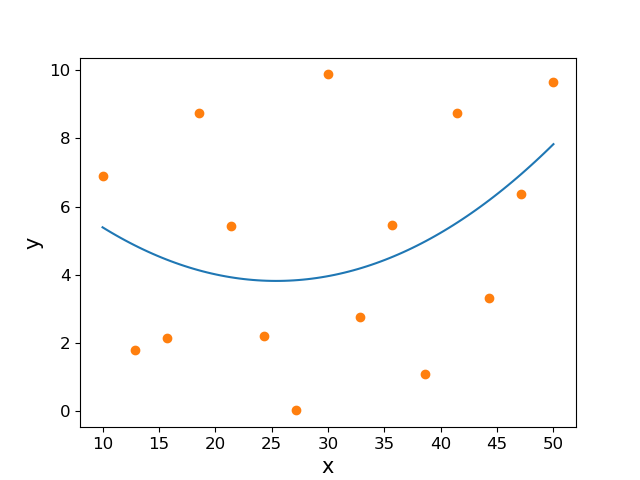
\includegraphics[width=\textwidth]{/Polynome/poly_deg2.png}
        \caption{Degree 2.}
        \label{fig:degree 2}
    \end{subfigure}
    \begin{subfigure}[b]{0.3\textwidth}
        \centering
        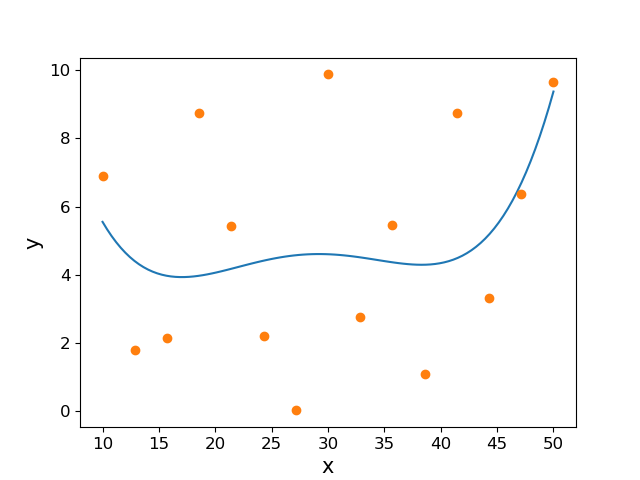
\includegraphics[width=\textwidth]{/Polynome/poly_deg4.png}
        \caption{Degree 4.}
        \label{fig:degree 4}
    \end{subfigure}
    \begin{subfigure}[b]{0.3\textwidth}
        \centering
        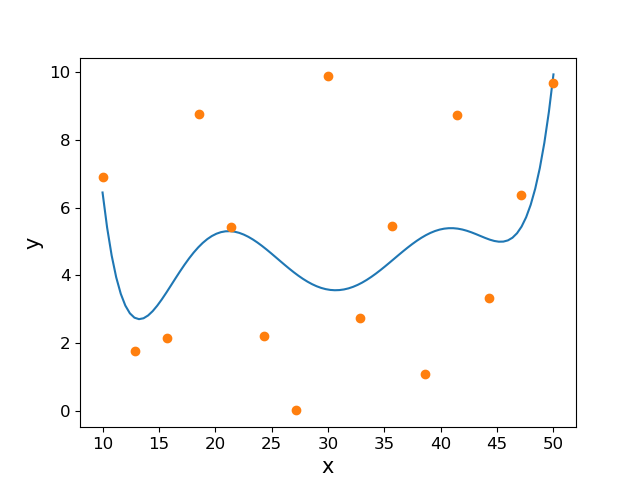
\includegraphics[width=\textwidth]{/Polynome/poly_deg6.png}
        \caption{Degree 6.}
        \label{fig:degree 6}
    \end{subfigure}
    \begin{subfigure}[b]{0.3\textwidth}
        \centering
        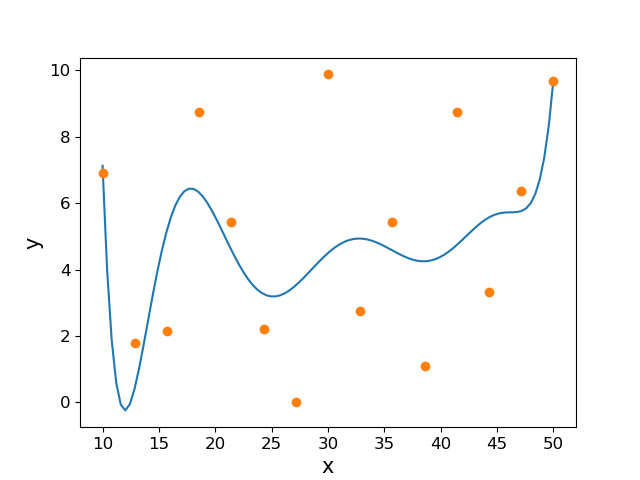
\includegraphics[width=\textwidth]{/Polynome/poly_deg8.png}
        \caption{Degree 8.}
        \label{fig:degree 8}
    \end{subfigure}
    \begin{subfigure}[b]{0.3\textwidth}
        \centering
        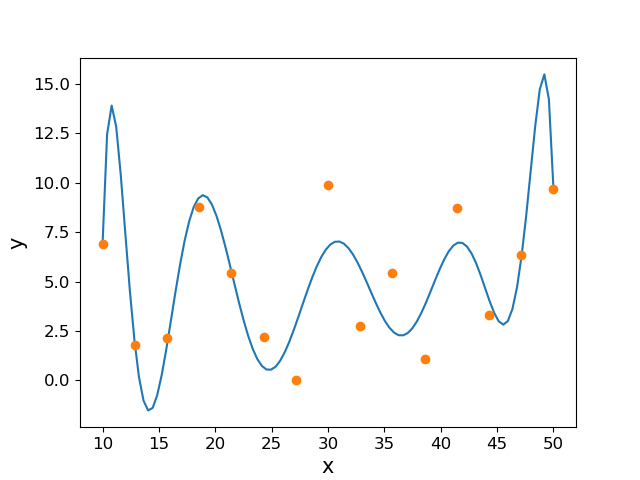
\includegraphics[width=\textwidth]{/Polynome/poly_deg10.png}
        \caption{Degree 10.}
        \label{fig:degree 10}
    \end{subfigure}
    \begin{subfigure}[b]{0.3\textwidth}
        \centering
        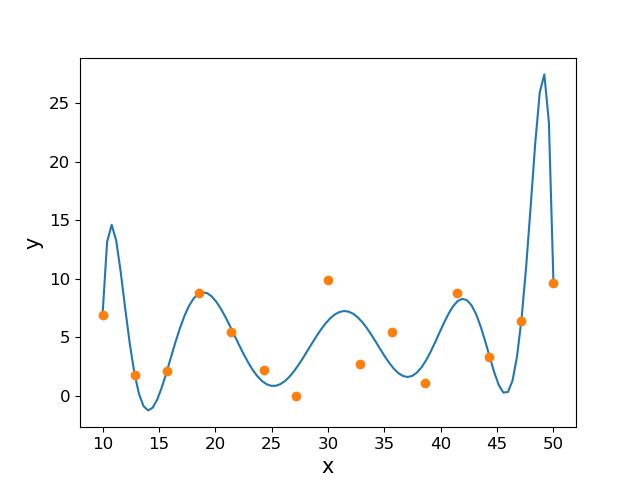
\includegraphics[width=\textwidth]{/Polynome/poly_deg12.png}
        \caption{Degree 12.}
        \label{fig:degree 12}
    \end{subfigure}
    \begin{subfigure}[b]{0.3\textwidth}
        \centering
        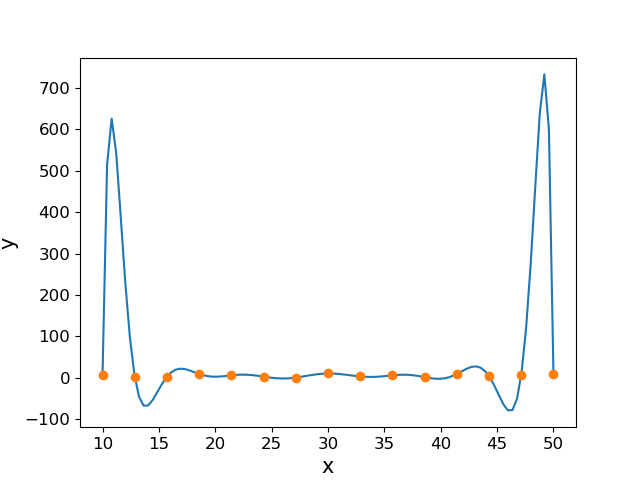
\includegraphics[width=\textwidth]{/Polynome/poly_deg14.png}
        \caption{Degree 14.}
        \label{fig:degree 14}
    \end{subfigure}
    \caption{Polynomial fitting of 15 points.} \label{fig:C7_poly}
\end{figure}

As illustrated in the series of schematics, when the highest degree of the polynomial increases, the amplitude of the variations increases as well. More precisely, the magnitude at the extremity of the domain defined by the set of points are the relatively large compared to the remaining of the function. 

Thus, it is required to minimize the degree of the polynomial to avoid these large fluctuation. This will be performed by  using the LS-R algorithm. The algorithm allows to restrict the maximal degree of the polynomial while keeping a good accuracy at the given points. For the remaining of the report, the abbreviation LS-RP will refer to the least-square regression algorithm using polynomials as basis functions.
\subsection{Splitting of the performance maps}
\quad\ When considering the performance maps of the compressor and the turbine, the range of value for the rotational speed can be becomes quite large. However, if the domain to be extrapolated by the polynomial is to wide, an evident loss of accuracy will occur. 

To avoid this loss of accuracy, it would be interesting to split the maps before applying the least-squares regression algorithm. Therefore, the polynomial will be defined by parts. However, there isn't any guaranty that the value of the polynomial at the junction of two parts will be the same. To solve this issue, each parts will be superimposed on each other. Then, a linear blending is perform to remove the discontinuity between the different parts. 

Considering two functions $f_1(x,N)$ and $f_2(x,N)$ superimposed for value of $N\in [N_{start},N_{end}]$, the blended function $f_{1,2}(x,N)$ is defined as follows:
\begin{equation}
 f_{1,2}(x,N) = \begin{cases}
f_1(x,N) &\text{ if }N<N_{start}\\
f_1(x,N) + f_2(x,N) - f_1(x,N))\cdot \alpha &\text{ if } N\in [N_{start},N_{end}]\\
f_2(x,N) &\text{ if }N>N_{end}
\end{cases}   
\end{equation}
where $\alpha$ is a coefficient for which its value is 0 for $N = N_{start}$ and 1 for $N = N_{end}$.  
\subsection{Compressor maps}
\quad\ First are considered the compressor maps. As it has been mentioned before, two functions need to be defined to fully characterized the compressor operating points.  
\subsubsection{Selection of the polynomial degree}
\quad\ To select the degree of the polynomial such that the function fit the best the given set of operating points, a parametric study over the maximal degree $d$ of the polynomial has been conducted. The data from Table \ref{tab:C7_compmap} will be used to perform this study.
For each of these polynomial, the value of the objective function $\textbf{F}$ and of the square of the residual function $Res^2$ are computed then compared. The results are expressed in Table \ref{tab:C7_regcomp}.

\begin{longtable}[c]{@{}lll|ll@{}}
\caption{Regression result - Compressor map (part 1 - Polynomial functions)}
\label{tab:C7_regcomp}\\
\toprule
                & \multicolumn{2}{l|}{$\Pi_{tt,c} = \Pi_{tt,c}(\dot{m}_{corr,c},N_c)$} & \multicolumn{2}{l}{$\eta_{is,c} = \eta_{is,c}(\Pi_{tt,c},N_c)$} \\* \midrule
\endfirsthead
%
\endhead
%
\bottomrule
\endfoot
%
\endlastfoot
%
\textbf{Degree} & \textbf{F}                     & $\mathbf{Res^2}$                    & \textbf{F}                  & $\mathbf{Res^2}$                  \\
\textbf{1}      & 0.104838                       & 0.745893                            & 0.073129                    & 0.780745                          \\
\textbf{2}      & 0.051117                       & 0.876103                            & 0.017796                    & 0.946643                          \\
\textbf{3}      & 0.028068                       & 0.93197                             & 0.008672                    & 0.973999                          \\
\textbf{4}      & 0.014399                       & 0.965099                            & 0.007718                    & 0.976861                          \\
\textbf{5}      & 0.008665                       & 0.978999                            & 0.007024                    & 0.97894                           \\
\textbf{6}      & 0.007111                       & 0.982765                            & 0.00668                     & 0.979973                          \\
\textbf{7}      & 0.006594                       & 0.984018                            & 0.006696                    & 0.979925                          \\* \bottomrule
\end{longtable}

From these results, several remarks can be drawn. First, the error with respect to the cloud of points when using polynomials of degree 1 or 2 is non negligible. For linear polynomials (degree 1), the square of the residual function is in average 25\% below the unity value, which is not acceptable. Considering now the quadratic polynomials (degree 2), the objective function can still be improve if polynomials of higher degree are used.

\begin{figure}[h]
    \setstretch{1}
    \centering
    \begin{subfigure}[b]{0.4\textwidth}
        \centering
        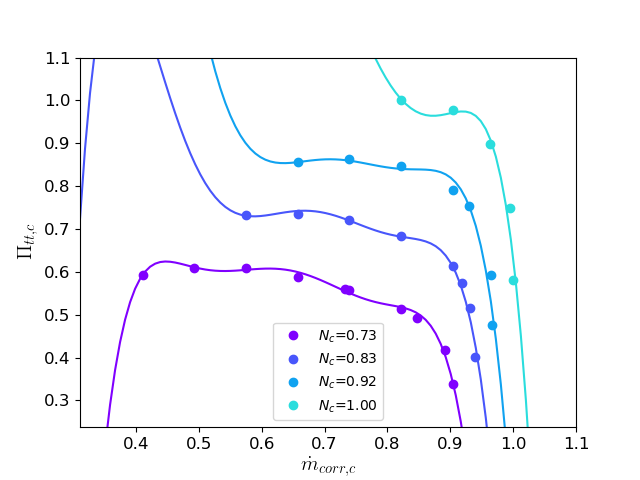
\includegraphics[width=\textwidth]{/Comp_map/calc_132_map.png}
        \caption{$\Pi_{tt,c} = \Pi_{tt,c}(\dot{m}_{corr,c},N_c)$}
        \label{fig:C7_polycomp1}
    \end{subfigure}
    \begin{subfigure}[b]{0.4\textwidth}
        \centering
        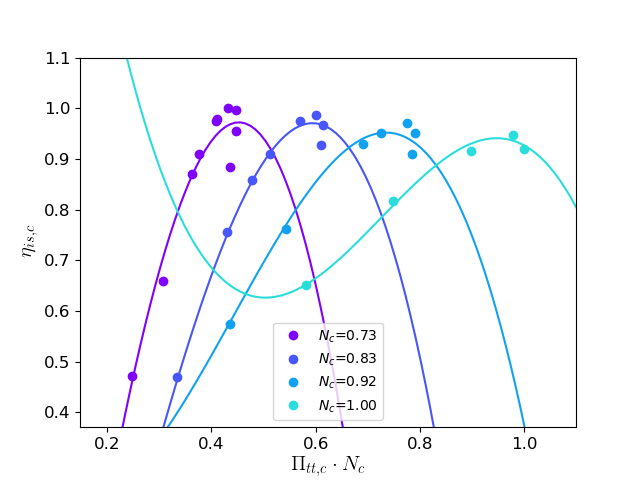
\includegraphics[width=\textwidth]{/Comp_map/calc_234_map.png}
        \caption{$\eta_{is,c} = \eta_{is,c}(\Pi_{tt,c},N_c)$}
        \label{fig:C7_polycomp2}
    \end{subfigure}
    \caption{Polynomial interpolation of the compressor.} \label{fig:C7_polycomp}
\end{figure}

Now, the choice of the maximal degree will depend on the relation. For the first one, it can be seen that there is no massive improvement of the residual function value for polynomials of degree greater than 6. Considering the second function, the analysis of the results shows that there is non interest of selecting polynomial of degree greater than 5.
On Figures \ref{fig:C7_polycomp1} and \ref{fig:C7_polycomp2} respectively depict the interpolating polynomial for the two relations.


\subsubsection{Extrapolation of the map at low RPM}
\quad\, When the compressor map is built, the low rotational speed operation points are usually not represented. However, at these low rotational speeds (below $\sim$ 40,000 RPM) the flow starts to behave as an incompressible flow. Therefore, the method of extrapolation of the performance maps seen for the pumps in chapter \ref{C4} can be applied on the map.

As expressed in the chapter \ref{C4}, two similar operating points $A$ and $B$ are linked by the relations (\ref{eq:C7_mdot}) to (\ref{eq:C7_eta}). 

\begin{subequations}
\setstretch{1}
\begin{align}
    \dot{Q}_{c,B} &= \dot{Q}_{c,A} \cdot \frac{N_{c,B}}{N_{c,A}}\nonumber\\
    \dot{m}_{corr,c,B} &= \dot{m}_{corr,c,A} \cdot \frac{N_{c,B}}{N_{c,A}}\label{eq:C7_mdot}\\
    \Delta h_{B}^0 &= \Delta h_{A}^0 \cdot \left(\frac{N_{c,B}}{N_{c,A}}\right)^2 \label{eq:C7_Dh}\\
    \eta_{is,c,B} &= \eta_{is,c,A} \label{eq:C7_eta}
\end{align}
\end{subequations}
with $\Delta h^0 = h_{2}^0 - h_{1}^0$, where the inlet and outlet states of the compressor are denoted \textbf{1} and \textbf{2}.\\

The extrapolation will assume that the gas used is air with constant
$c_p=1005 J/kg*K$ and $r = 287 J/kg*K$. 

To initialize the method, reference conditions needs to be defined:

\begin{align*}
    \setstretch{1}
    T_{0}^0 & = 293.15K\\
    h_{0}^0 & = \int_{T_{0}^0}^{T_{0}^0} c_p dT = 0\\
    r & = 287 \text{ J/(kg$\cdot$ K)}\\
    k &= \frac{c_p - r}{c_p} = 1.4
\end{align*}
Then, considering the known operating point $A$, the variation of the enthalpy $\delta_{A}^0$ is obtained  following the relations seen in the section \ref{C3:Isen_eff} are used. The mathematics development are expressed in (\ref{eq:C7_DhA}), where the inlet condition $1$ of the compressor corresponds to the reference conditions specified above.

\begin{align}
\setstretch{1}
    T_{A,1}^0 = T_{0}^0 &\text{ and } h_{A,1}^0 = T_{0}^0\nonumber\\
    \frac{T_{A,2,is}^0}{T_{A,1}^0} &= \left(\Pi_{tt,c,A}\right)^{\frac{k-1}{k}}\nonumber\\
    T_{A,2}^0 &= T_{A,1}^0 + \frac{T_{A,2,is}^0 - T_{A,1}^0}{\eta_{is,c,A}}\label{eq:C7_DhA}\\
    h_{A,2}^0 &= h_{0}^0 + c_p\cdot (T_{A,2}^0 - T_{0}^0)\nonumber\\
    \Rightarrow \Delta h_A^0 &= h_{A,2}^0  - h_{A,1}^0\nonumber
\end{align}

Once the enthalpy variation $\Delta h_A^0$ is computed, the one for the similar operating point $B$ can be obtained from the relation (\ref{eq:C7_Dh}).

Then, the total to total pressure ratio produced by the compressor at the operating point $B$ by applying backward the relations of (\ref{ea:C7_DhA}). Therefore, the following development (\ref{eq:C7_DhB} can be derived.

\begin{align}
\setstretch{1}
    T_{B,2}^0 = T_{0}^0 &\text{ and } h_{B,2}^0 = T_{0}^0\nonumber\\
    h_{B,2}^0 &= \Delta h_B^0 + h_{B,1}^0\nonumber\\
    T_{B,2}^0 &= \frac{h_{B,2}^0 - h_{0}^0}{c_p} + T_0^0\label{eq:C7_DhB}\\
    T_{B,2,is}^0 &= \left(T_{B,2}^0 - T_{B,1}^0\right)\cdot \eta_{is,c,B} + T_{B,1}^0\nonumber\\
    \Pi_{tt,c,B} &= \left(\frac{T_{B,2,is}^0}{T_{B,1}^0}\right)^{\frac{k}{k-1}}\nonumber
\end{align}
Using this method, low rotational speed operating points can be derived and used to improve the accuracy of the polynomial regression.

\subsection{Delimitation of the compressor map domain}
\quad\ While it has been expressed previously that polynomial of high degree are not reliable at the extremity of the domain defined by the given set of operating points, this doesn't really matter here since the domain of operation of the compressor is naturally limited by the choke and surge lines described in the chapter \ref{C4}.

Several methods are going to be presented in this part of the section dedicated to the modeling of the turbomachines. 
\subsubsection{Triangulation without constraints}
To implement these limits into the model, different methods have been studied. The first method consisted in creating a triangular meshing not constraint through the couple of points $(\dot{m}_{corr,c},\Pi_{tt,c})$. This method has some advantages with first the rapidity of the method. Indeed, it does not take lots of computer resources to generate the mesh. Also, once the triangles created, the algorithm to check if the operating point is inside or outside the domain is really easy.

However, there are serious flaws that makes the method unusable for the targeted application. Indeed, while the method gives easy tools to reject or not an operating point, finding the coordinates $(\dot{m}_{corr,c},\Pi_{tt,c})$ of the boundary for a given rotational speed is more tricky. 

The other weakness of the triangulation method is that it only works well with convex hull. The reason behind is that during the triangulation process, the program building the triangle does not know how the points are linked together. Unfortunately, some sections of the compressor map are not convex but concave. Therefore, when performing the triangulation, the concavity disappear and the resulting mesh exceed the real envelop of the map.

\begin{figure}[h]
    \centering
    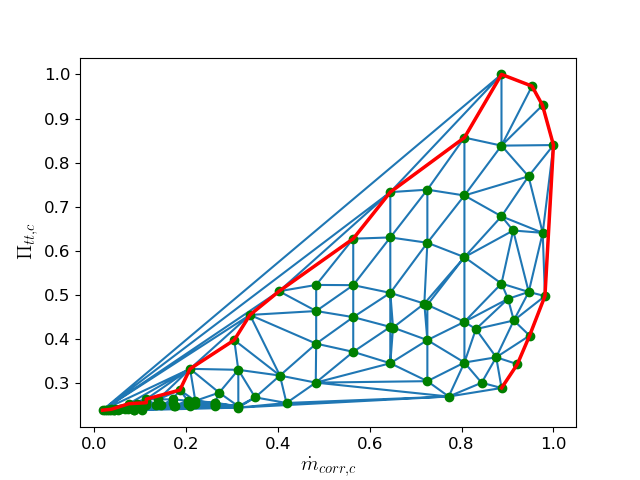
\includegraphics[width=0.5\textwidth]{/Comp_map/map_triang.png}
    \caption{Simple triangulation of the compressor map}
    \label{fig:C7_trimap}
\end{figure}

Figure \ref{fig:C7_trimap} depicts the result of the triangulation of the compressor map. In red is represented the compressor map boundary, and in green the meshing. The time taken to create the mesh is equal to 2.5ms.

As it can be seen on the graph, the surge line is misrepresented by the mesh. The limit provided by the triangulation is very optimistic and doesn't correspond with the reality. 

\subsubsection{Triangulation with constraints}
\quad\ As explained in last lines, the basic triangulation method cannot handle concave hull by itself. In order to take into consideration these shapes, some conditions have to be set to reject or not the triangle of the mesh. A selection algorithm  has been developed \cite{} based on the geometry of the triangle.

To illustrate the algorithm, the triangle with its circumscribed circle on Figure \ref{fig:C7_triangmesh} can be considered.

\begin{figure}[h]
    \centering
    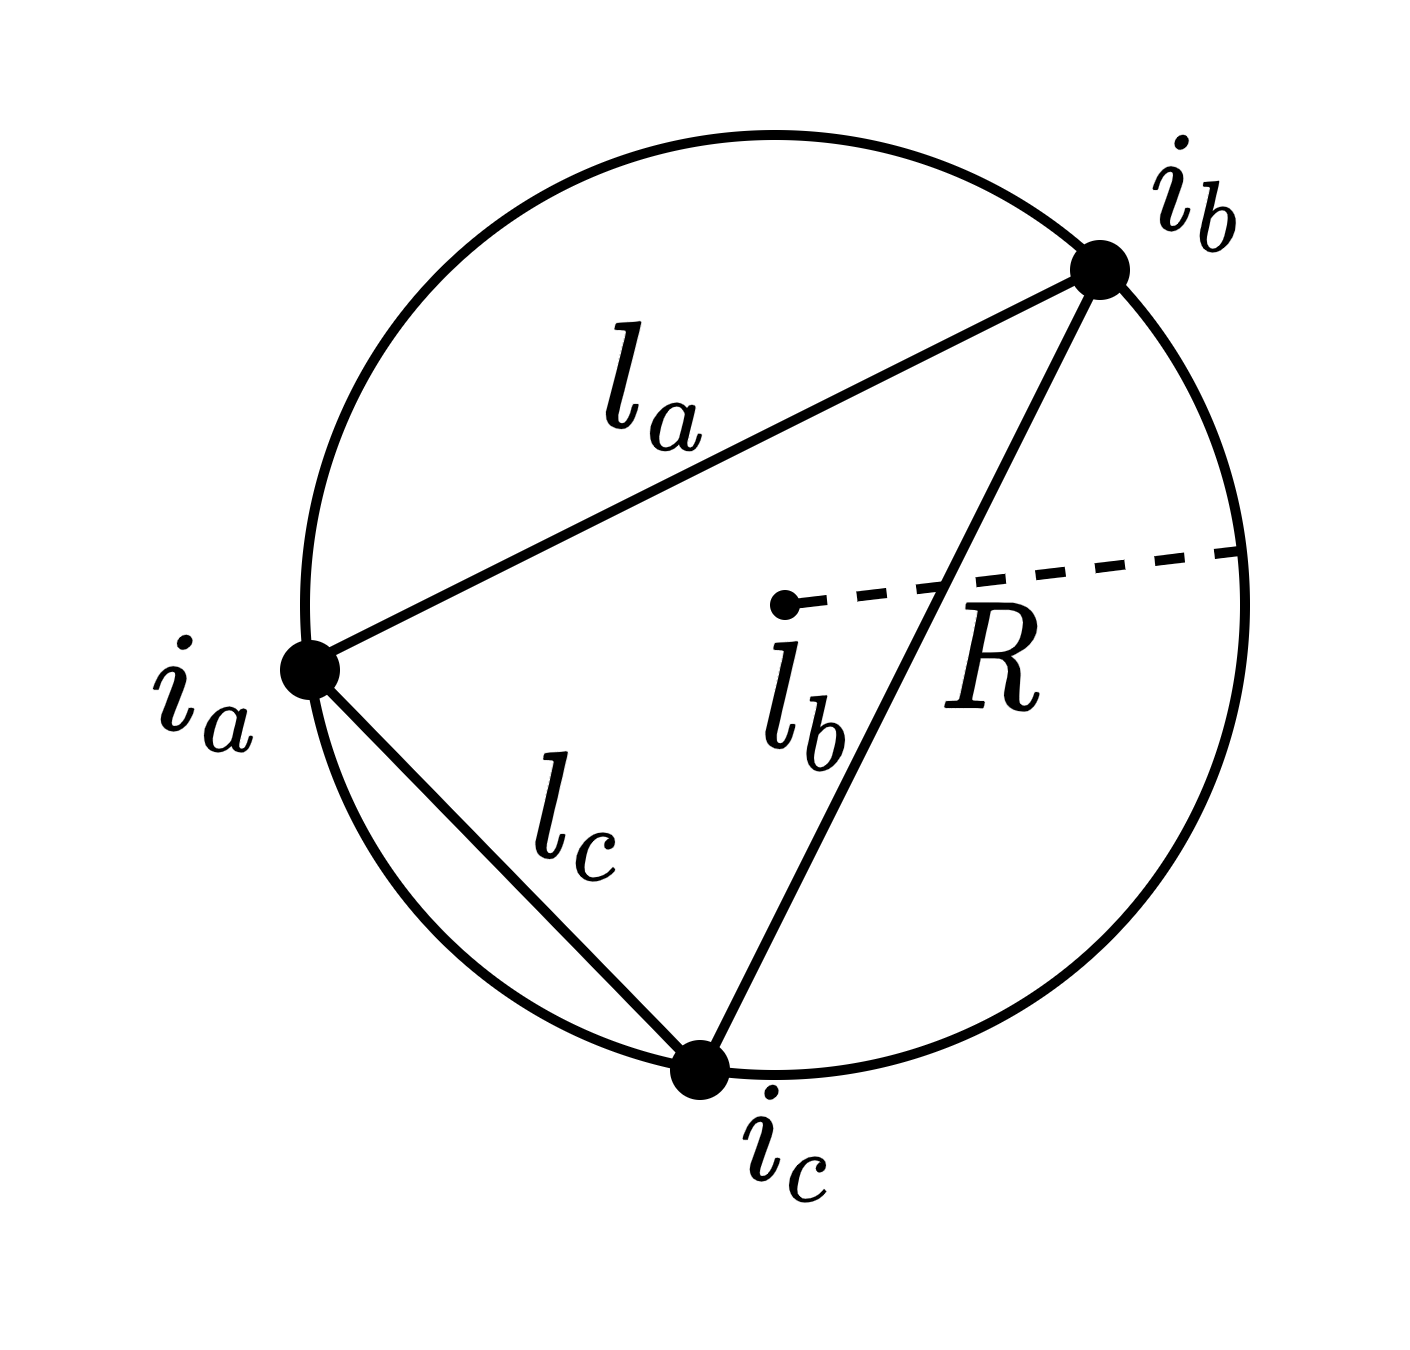
\includegraphics[width=0.4\textwidth]{Comp_map/triang_mesh.png}
    \caption{Triangle with its coordinates within the mesh}
    \label{fig:C7_triangmesh}
\end{figure}

The three nodes $i_a$, $i_b$ and $i_c$ are respectively characterized by the coordinates $(x_a,y_a)$, $(x_b,y_b)$, $(x_c,y_c)$. Using the coordinates, the length of the triangle edges are computed as follows.

\begin{align*}
    \setstretch{1}
    l_a &= \sqrt{(x_a - x_b)^2 + (y_a - y_b)^2}\\
    l_b &= \sqrt{(x_b - x_c)^2 + (y_b - y_c)^2}\\
    l_c &= \sqrt{(x_c - x_a)^2 + (y_c - y_a)^2}
\end{align*}
Then, the intermediary quantity $s$, called simeperimeter, is computed using the formula (\ref{eq:C7_semiperim}).

\begin{equation}
    \setstretch{1}
    s = \frac{a + b + c}{2}\label{eq:C7_semiperim}
\end{equation}
Using $l_a$, $l_b$, $l_c$, and $s$, the radius $circ_R$ of the circumscribed circle can be calculated using the relation (\ref{eq:C7_circum}). 

\begin{equation}
    \setstretch{1}
   circ_r = \frac{a\cdot b\cdot c}{4\cdot \sqrt{s\cdot (s - l_a)\cdot (s - l_b)\cdot (s - l_c)}}\label{eq:C7_circum}
\end{equation}

Now that the radius of the circumscribed circle of the triangle have been computed, the triangle will be rejected if the condition $circ_r <\frac{1}{\alpha}$ is not satisfied. This condition is justified by noting that for triangles outside the envelope, the radius will likely be bigger since all these triangles are obtuse. The parameter $\alpha$ needs to be tuned in order to eliminate the triangles outside the concave hull. 

The series of Figures \ref{fig:C7_alpha} illustrates the triangle mesh considering different values for the parameter $\alpha$.

\begin{figure}[h]
    \setstretch{1}
    \centering
    \begin{subfigure}[b]{0.3\textwidth}
        \centering
        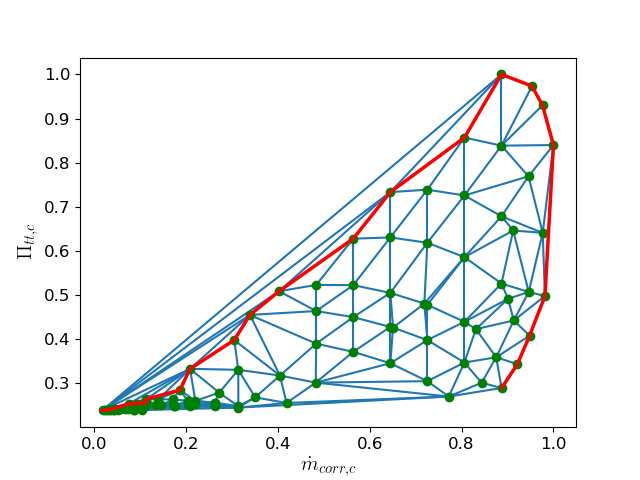
\includegraphics[width=\textwidth]{/alpha/map_triang0_0.png}
        \caption{$\alpha=0$.}
        \label{fig:alpha0}
    \end{subfigure}
    \begin{subfigure}[b]{0.3\textwidth}
        \centering
        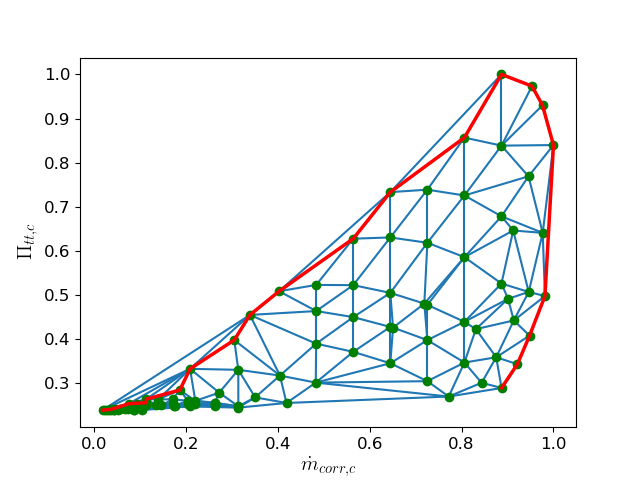
\includegraphics[width=\textwidth]{/alpha/map_triang1_0.png}
        \caption{$\alpha=1$.}
        \label{fig:alpha1}
    \end{subfigure}
    \begin{subfigure}[b]{0.3\textwidth}
        \centering
        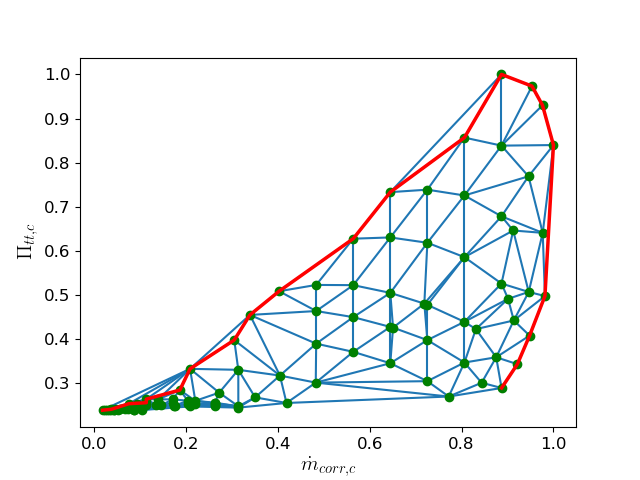
\includegraphics[width=\textwidth]{/alpha/map_triang2_0.png}
        \caption{$\alpha=2$.}
        \label{fig:alpha2}
    \end{subfigure}
    \begin{subfigure}[b]{0.3\textwidth}
        \centering
        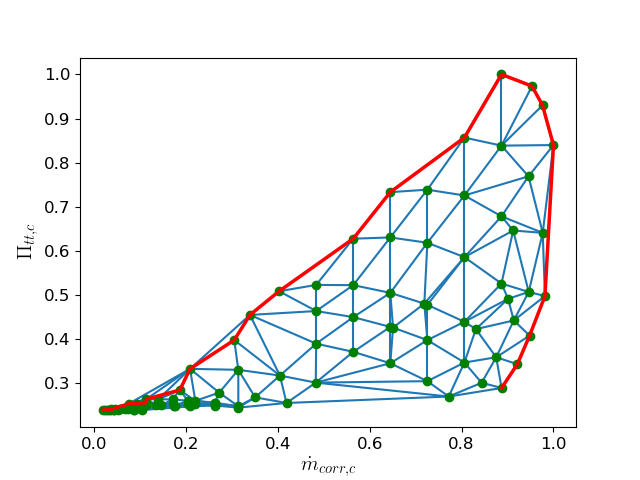
\includegraphics[width=\textwidth]{/alpha/map_triang3_0.png}
        \caption{$\alpha=3$.}
        \label{fig:alpha3}
    \end{subfigure}
    \begin{subfigure}[b]{0.3\textwidth}
        \centering
        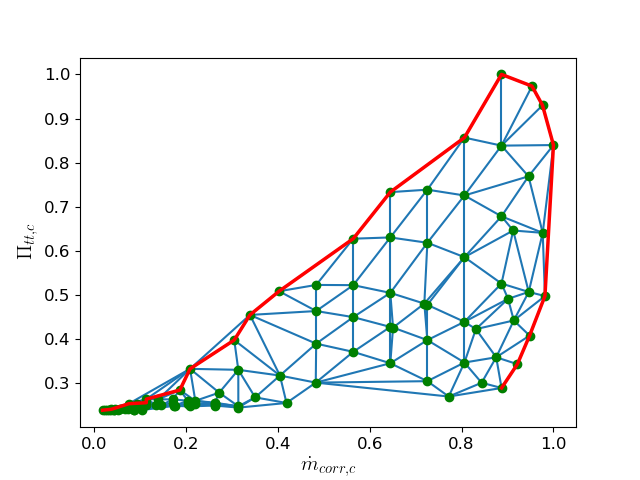
\includegraphics[width=\textwidth]{/alpha/map_triang4_0.png}
        \caption{$\alpha=4$.}
        \label{fig:alpha4}
    \end{subfigure}
    \begin{subfigure}[b]{0.3\textwidth}
        \centering
        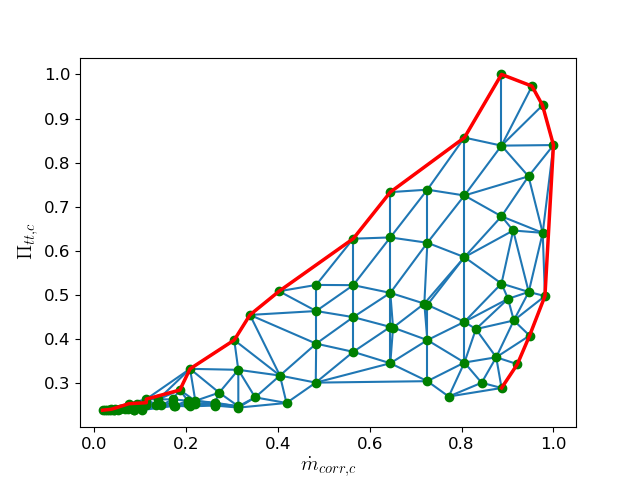
\includegraphics[width=\textwidth]{/alpha/map_triang5_0.png}
        \caption{$\alpha=5$.}
        \label{fig:alpha5}
    \end{subfigure}
    \begin{subfigure}[b]{0.3\textwidth}
        \centering
        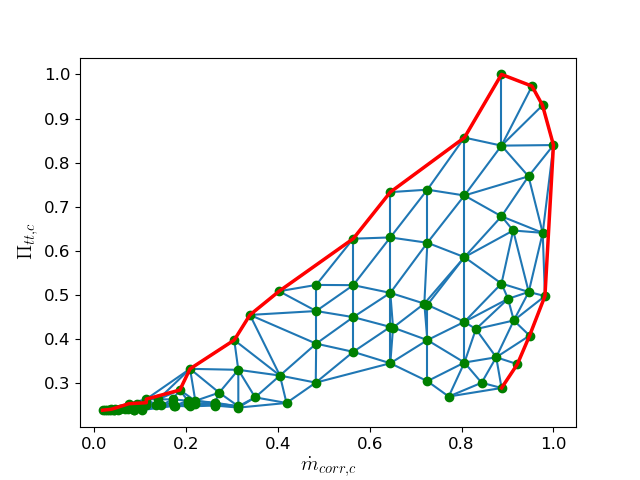
\includegraphics[width=\textwidth]{/alpha/map_triang6_0.png}
        \caption{$\alpha=6$.}
        \label{fig:alpha6}
    \end{subfigure}
    \begin{subfigure}[b]{0.3\textwidth}
        \centering
        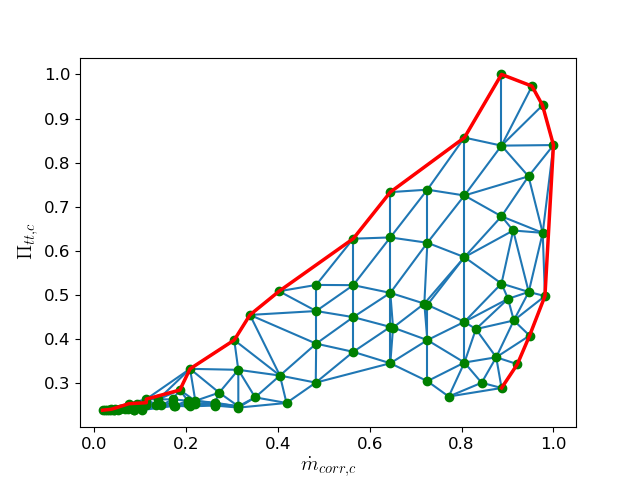
\includegraphics[width=\textwidth]{/alpha/map_triang7_0.png}
        \caption{$\alpha=7$.}
        \label{fig:alpha7}
    \end{subfigure}
    \begin{subfigure}[b]{0.3\textwidth}
        \centering
        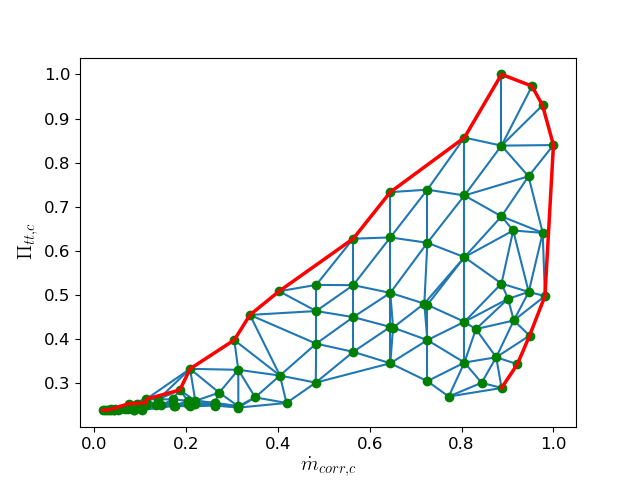
\includegraphics[width=\textwidth]{/alpha/map_triang8_0.png}
        \caption{$\alpha=8$.}
        \label{fig:alpha8}
    \end{subfigure}
    \caption{Triangulation with triangle selection condition.} \label{fig:C7_alpha}
\end{figure}

The picture \ref{fig:alpha3} shows that for $\alpha=3$, most of the triangles outside the map domain are rejected. However, for the low pressure ratio it still remains some non desired artifacts. Increasing the value of the $\alpha$ would allow to reject these
triangles as well but, some triangles within the domain also start to be removed. So, the value $\alpha=3$ is a good compromise.

\subsubsection{2D level-set}
\quad\ The triangulation with a condition to select the triangles provides relatively good results. However, this method is not really robust because each times a new map is provided to the program, the value of the $\alpha$ has to be tuned by hand. An automatic method would consist in defining a level-set function that would delimit the performance map domain.

First has been considered a 2 dimensional function defined by the coordinates $(\dot{m}_{corr,c},\Pi_{tt,c})$ of the boundary points of the map. To built this function, a linear interpolation between these points have been used. Linear interpolation is chosen to have an interpolated surge line that is more restrictive that the actual surge line.

On Figure \ref{fig:C7_LS2D} is represented the level set function.

\begin{figure}[h]
    \centering
    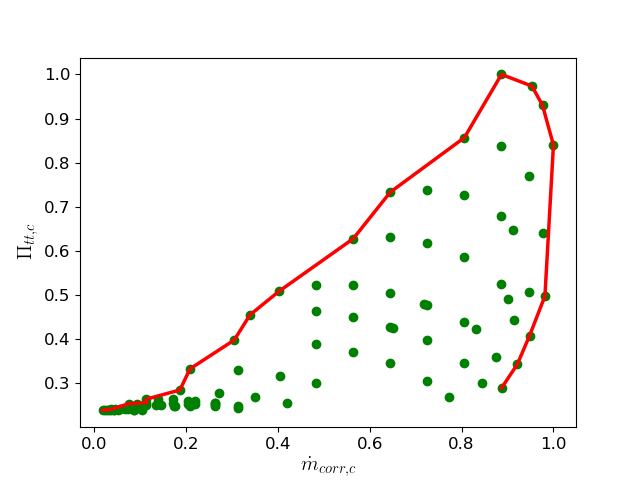
\includegraphics[width=0.6\textwidth]{Comp_map/2D_LS.png}
    \caption{2D level-set function.}
    \label{fig:C7_LS2D}
\end{figure}

Compared to the triangulation, the computation of the boundary coordinates for a given rotational speed $N_c$ can easily be found by determining the intersection points between the level-set function $f_{ls,2D}$ and the interpolation function $\Pi_{tt,c} = \Pi_{tt,c}(\dot{m}_{corr,c},N_c)$. 
However, this 2D level-set function needs to be defined by parts since for some value of mass flow rate $\dot{m}_{corr,c}$, there exist two corresponding values for the pressure ratio $\Pi_{tt,c}$. Also, the data need to be pre-processed to only retained the boundary points of the maps. 

\subsubsection{3D level-set}
\quad\ The two cons of the 2D level-set can be erased by considering a 3D level-set. Here, the principle then to be closed to the performance maps regressions described in the previous parts of this section. However, here what is desired is a function defined inside the cloud of points and equal to the NULL value outside the cloud. 

The relation used to build the 3D level-set function $f_{ls,3D}$ is $\dot{m}_{corr,c} = \dot{m}_{corr,c}(\Pi_{tt,c},N_c)$. On Figure \ref{fig:C7_LS3D} is illustrated this level-set function. A 

\begin{figure}[h]
    \centering
    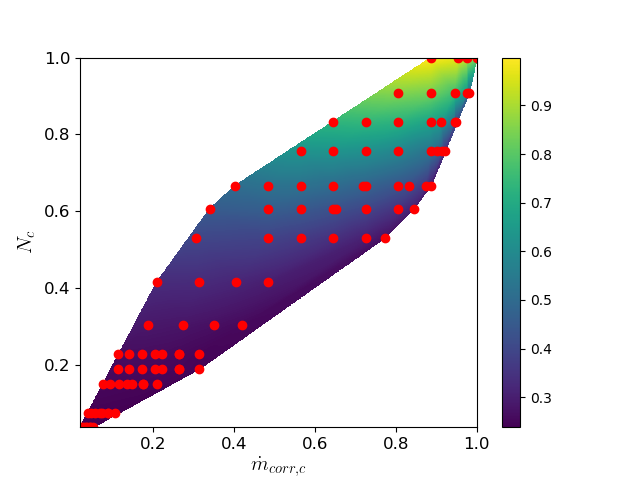
\includegraphics[width=0.6\textwidth]{Comp_map/3D_LS.png}
    \caption{3D level-set function - color bar representing the value of the pressure ratio.}
    \label{fig:C7_LS3D}
\end{figure}
For each rotational speed $N_c$, the function gives all the admissible couples $(\dot{m}_{corr,c},\Pi_{tt,c})$ based on the compressor map initially provided. 

Considering first the surge line, the limit drawn by the function is relatively faithful regarding to what was expected. If some margins is applied, the surge line can be nicely characterized by this 3D level-set function. 

\subsection{Estimation of the choke line}
\quad\ The choke lines can be defined by the 3D level-set function as well but, an alternative solution using the least-square regression algorithm can be consider.


In chapter \ref{C4}, it has been explained that the relation $\Pi_{tt,c}(\dot{m}_{corr,c},N_c)$ is characterized by an infinite slope when the compressor is choking. However, the polynomial built using the least-square regression algorithm is not designed to represent infinite slope. Indeed, the polynomials composed of monomial of degree greater than zeros don't have any asymptotic behavior.

If the inverse relation $\dot{m}_{corr,c}(\Pi_{tt,c},N_c)$ is considered instead, the choke limit will happen when the derivative of the function will be equal to zeros. To select the degree of the polynomial, a parametric study have been conducted. The results in Table \ref{tab:C7_regcomp2} shows that a polynomial of degree 4 should be selected.

\begin{longtable}[c]{@{}lll@{}}
\caption{Regression result - Compressor map (part 2 - Polynomial functions)}
\label{tab:C7_regcomp2}\\
\toprule
                & \multicolumn{2}{l}{$\dot{m}_{corr,c} = \dot{m}_{corr,c}(\Pi_{tt,c},N_c)$} \\* \midrule
\endfirsthead
%
\endhead
%
\bottomrule
\endfoot
%
\endlastfoot
%
\textbf{Degree} & \textbf{F}                       & $\mathbf{Res^2}$                       \\
\textbf{1}      & 0.104838                         & 0.745893                               \\
\textbf{2}      & 0.051117                         & 0.876103                               \\
\textbf{3}      & 0.028068                         & 0.93197                                \\
\textbf{4}      & 0.014399                         & 0.965099                               \\
\textbf{5}      & 0.008665                         & 0.978999                               \\
\textbf{6}      & 0.007111                         & 0.982765                               \\
\textbf{7}      & 0.006594                         & 0.984018                               \\* \bottomrule
\end{longtable}

\begin{figure}[h]
    \centering
    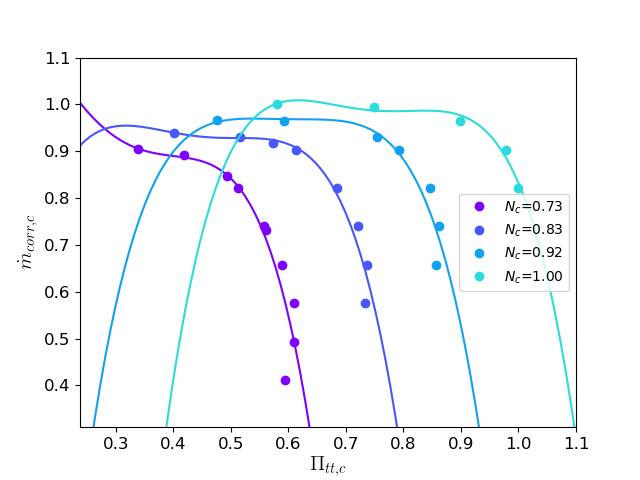
\includegraphics[width=0.6\textwidth]{Comp_map/calc_231_map.png}
    \caption{$\dot{m}_{corr,c}(\Pi_{tt,c},N_c)$ - polynomial function.}
    \label{fig:C7_polycomp3}
\end{figure}

However, It can be noticed on Figure \ref{fig:C7_polycomp3} depicting the polynomial function that, for a given rotational speed $N_c$, there are several values of $\Pi_{tt,c}$ for which the derivative of the function is equal to zeros. Therefore, it would be difficult to apply a systematic rule to determined the corrected mass flow rate at which the machine is choking. 

If the degree of the polynomial is decreased such that the number of minimum/maximum is smaller, the fitting function will loose too much in accuracy to stay reliable. Therefore, for this particular application polynomial are not good enough.

An alternative to polynomials would be trigonometric functions. These functions are characterized by linear combination of cosinus and sinus. Here, the degree is no longer the maximal exponent but rather the maximal factor multiplying the variable within the trigonometric functions. An example of degree 2 trigonometric function is given in (\ref{eq:C7_trigo}).

\begin{align}
\setstretch{1}
    f(x,y) &= a_{1,1} + a_{1,2}\cdot sin(y) + a_{1,3}\cdot cos(y) + a_{1,4}\cdot sin(2\cdot y) + a_{1,5}\cdot cos(2\cdot y)\nonumber\\
           &+ a_{2,1}\cdot sin(x) + a_{2,2}\cdot sin(x)\cdot sin(y) + a_{2,3}\cdot sin(x)\cdot cos(y)\nonumber\\
           &+ a_{3,1}\cdot cos(x) + a_{3,2}\cdot sin(y)\cdot cos(x) + a_{3,3}\cdot cos(x)\cdot cos(y)\label{eq:C7_trigo}\\
           &+ a_{4,1}\cdot sin(2\cdot x)\nonumber\\
           &+ a_{5,1}\cdot cos(2\cdot x) \nonumber
\end{align}

As for the polynomial function, a study on the degree have been performed. The results, expressed in Table \ref{tab:reg_compmap3}, shows that a trigonometric function of degree 2 is the best choice to be made. The Figure \ref{fig:C7_trigo} depicts the fitting function for the rotational speed specified in the data.

\begin{longtable}[c]{@{}lll@{}}
\caption{Regression result - Compressor map (part 3 - Trigonometric functions).}
\label{tab:reg_compmap3}\\
\toprule
                & \multicolumn{2}{l}{$\dot{m}_{corr,c} = \dot{m}_{corr,c}(\Pi_{tt,c},N_c)$} \\* \midrule
\endfirsthead
%
\endhead
%
\bottomrule
\endfoot
%
\endlastfoot
%
\textbf{Degree} & \textbf{F}                       & $\mathbf{Res^2}$                       \\
\textbf{1}      & 0.113446                         & 0.677763                               \\
\textbf{2}      & 0.02983                          & 0.915268                               \\
\textbf{3}      & 0.028411                         & 0.919299                               \\
\textbf{4}      & 0.028243                         & 0.919777                               \\
\textbf{5}      & 0.027913                         & 0.920714                               \\* \bottomrule
\end{longtable}

\begin{figure}[h]
    \centering
    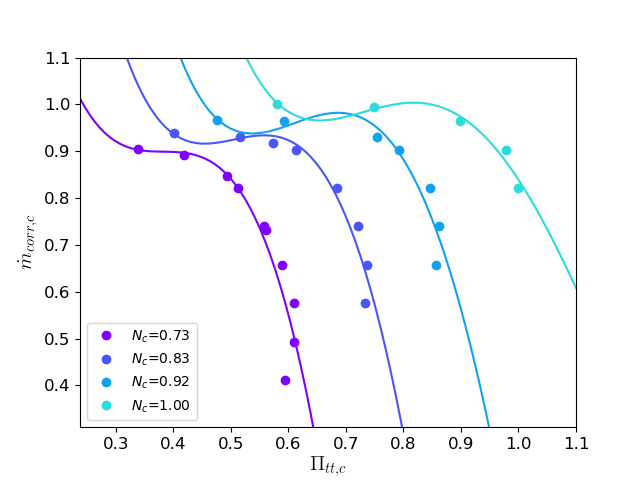
\includegraphics[width=0.6\textwidth]{Comp_map/calc_231_map_trigo.png}
    \caption{$\dot{m}_{corr,c}(\Pi_{tt,c},N_c)$ - trigonometric function}
    \label{fig:C7_trigo}
\end{figure}

Here, it can be noticed that the function systematically goes through a local minimum before going up to the infinity for decreasing values of the pressure ratio $\Pi_{tt,c}$. Thus, the flow rate at which the compressor start to choke can be set at the value of the function at that local minimum. 

\subsection{Turbine maps}


